\chapter{VARIATIONAL AUTOENCODERS}
\label{chapter:vae}
\begin{onehalfspacing}
    \section{The Standard Autoencoder}
    Autoencoders are unsupervised neural networks that can learn efficient 
    data encodings. Autoencoders learn the representation for the data, 
    typically for dimensionality reduction. Initially, an autoencoder 
    compresses the input data into a latent vector. The latent vector can be 
    used to regenerate the input data later. Traditionally, autoencoders were 
    used for dimensionality reduction and feature learning. In the recent times, 
    autoencoders are being used to learn generative models of data.

    \begin{figure}[h]
        \centering
        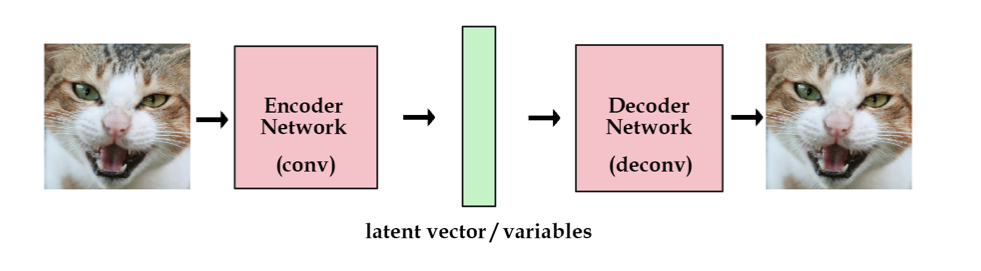
\includegraphics[width=0.8\linewidth]{images/autoencoders.png}
        \caption{Autoencoders \cite{autoencoders_kvfrans}}
        \label{fig:autoencoders}
    \end{figure} 

    As shown in figure \ref{fig:autoencoders}, the autoencoder has two 
    component neural networks, an encoder and a decoder. The encoder neural 
    network can be represented by $h = f(x)$ and it takes the input image and 
    encodes it into a latent vector. The decoder, $r = g(h)$ then produces a 
    reconstruction. An autoencoder will be not useful if it simply replicates 
    the input given to it. Thus, the autoencoder is not allowed to copy the 
    input directly instead it learns useful parameters from the 
    input \cite{dlbook}.

    \section{Variational Autoencoder}
    
    We cannot create a new image using a standard autoencoder since the 
    latent vectors are obtained by encoding an input image. We can make an 
    autoencoder create new images by adding a constraint to the encoder neural 
    network. A variational autoencoder differs from a standard one by the fact 
    that the encoder of the variational autoencoder is forced to create latent 
    vectors that roughly follow a unit Gaussian distribution. For generating 
    new images, we can sample new latent vectors from the Gaussian distribution 
    and pass it onto the decoder.
    In practice, there is a tradeoff between how exactly the sampled latent 
    vector matches the Gaussian distribution and how accurate our network is.

    The loss function of the autoencoder has two components. They are the 
    generative loss and the latent loss. The generative loss estimates the 
    mean squared error of how accurately the network regenerated the image. 
    The latent loss is the Kullback$-$Leibler divergence 
    \footnote{In mathematical statistics, Kullback$-$Leibler divergence 
    (also called as relative entropy) measures how one probability distribution 
    differs from another. \cite{kldiv_wiki}} that measures how 
    closely the latent variables match the Gaussian distribution 
    \cite{autoencoders_kvfrans}.
    \\
    \\
    \textit{generation loss = mean squared error between generated image 
    and real image}
    \\
    \textit{latent loss = KL-Divergence between latent variable and unit Gaussian}
    \\
    \textit{total loss = generation loss + latent loss}

    \begin{figure}[h]
        \centering
        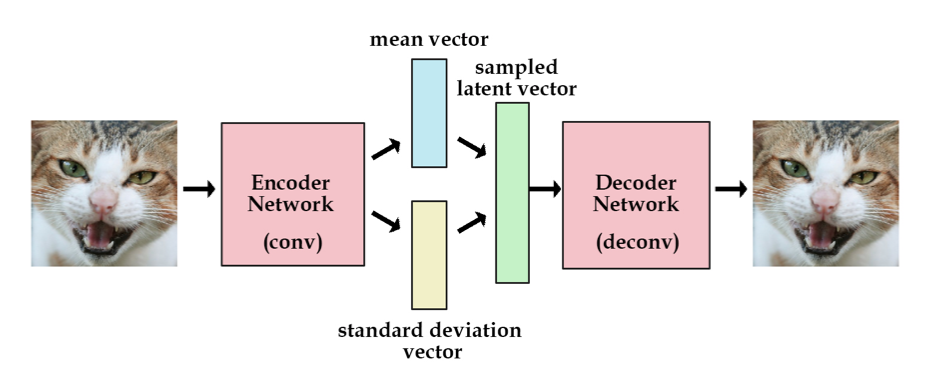
\includegraphics[width=0.8\linewidth]{images/vae_kl_div.png}
        \caption{Optimizing KL divergence for variational 
        autoencoders \cite{autoencoders_kvfrans}}
        \label{fig:vae}
    \end{figure} 

    As shown in figure \ref{fig:vae}, if the encoder generates a vector of means 
    and standard deviations, we can optimize KL divergence. This report will 
    discuss the performance of Variational Autoencoders and its comparison with 
    GANs in chapter \ref{chapter:conclusion}.

\end{onehalfspacing}